\documentclass[12pt,a4paper]{article}

\usepackage[utf8]{inputenc}
\usepackage[T1]{fontenc}
\usepackage[top=3cm, bottom=4.5cm, left=2.8cm, right=2.8cm]{geometry}
\usepackage[pdftex]{graphicx}
\usepackage[italian]{babel}
\usepackage{bold-extra, amssymb, amsmath, mathtools, microtype, cite}
\usepackage{subcaption}
\usepackage{wrapfig}
\usepackage{relsize}
\usepackage{rotating}
\usepackage{colortbl}
\usepackage{color}
\usepackage{siunitx}
\usepackage{textcomp}
\usepackage{paracol}
\usepackage{fancyhdr}
\usepackage{svg}
\usepackage{hyperref}

\svgpath{{images/}}
\graphicspath{{images/}}

\pagestyle{fancyplain}
\headheight 35pt
\lhead{Politecnico di Torino}
%\chead{\today}
\rhead{Tecnologie per IoT}
\lfoot{}
\cfoot{}

\begin{document}

\begin{figure}[b]
\centering
\includesvg[width=0.2\textwidth]{logo_polito}
\end{figure}

%\begin{vplace}[0.15]
\title{Relazione laboratorio Hardware}
\author{}
\maketitle
%\begin{center}
%    \LARGE{\textbf{Relazione Laboratorio Hardware}}
%\end{center}
\vspace{10cm}
\begin{center}Davide Miola\\Elia Fontana\end{center}
%\end{vplace}

\newpage
\setcounter{page}{1}
\rfoot{\thepage}
%\thispagestyle{myheadings}
\section{Introduzione}

Per prima cosa, data la situazione straordinaria nella quale il corso, ed in particolare i laboratori, si sono dovuti svolgere, si ritiene opportuno premettere qualche parola su come il gruppo si è organizzato e come le consegne sono state eseguite in remoto.
\\ \\
Durante ogni orario di lezione in cui si è tenuto un laboratorio, i componenti del gruppo si sono collegati in una videochiamata utilizzando il software gratuito Skype; Davide Miola, che ha ricevuto il kit con tutta la strumentazione dal Politecnico, utilizzando una webcam montata precariamente su di una lampada, ha cercato di inquadrare, per quanto possibile, la zona di lavoro con l'Arduino. Nonostante gli sforzi, tuttavia, è risultato quantomai difficile ottenere un'esperienza realmente interattiva tra i due membri del gruppo: chi aveva la scheda di fronte a sè poteva scrivere il codice condividendo il proprio schermo al compagno in remoto, il quale però non poteva che commentare e dare consigli.

Terminato l'orario di lezione in programma per il corso, il gruppo ha spesso continuato a svolgere l'attività di laboratorio per parecchi minuti successivi, oltre ad essere riuscito a riunirsi talvolta in sessioni al di fuori degli orari ufficiali.
\\ \\
Inoltre, ogni riga di codice scritta per il laboratorio è stata condivisa sia in diretta, sia su una repository Github appositamente creata. In questo modo, il software sviluppato poteva essere consultato liberamente do ogni membro del gruppo, in ogni momento.
\\ \\
In aggiunta, ci tengo a menzionare che, per scrivere il codice C++ per la Yùn Rev2, si è impiegato l'eccellente IDE open source \textit{Visual Studio Code}, con l'estensione ufficiale di Microsoft per il supporto alla programmazione delle schede Arduino o compatibili. Così, si è potuto sfruttare non solo il \textit{syntax highlighting} per il linguaggio, peraltro presente anche sull'IDE ufficiale, ma anche il motore \textit{Intellisense} per il completamento automatico del codice.

L'IDE ufficiale è stato pertanto abbandonato quasi del tutto, se non per qualche piccolo dettaglio quale l'impossibilità, per l'estensione di VS Code, di modificare il terminatore di riga per l'invio di stringhe tramite interfaccia seriale.

\newpage
\section{Prima Parte}

La prima sezione del laboratorio di hardware è stata molto guidata; in particolare il primo esercizio, che per i sottoscritti è coinciso con l'assoluto primo contatto con il mondo Arduino e, in generale, con la programmazione \textit{embedded}, è stato risolto seguendo le indicazioni del professor Pagliari.
\\ \\
Il secondo esercizio vede l'introduzione della comunicazione seriale: ad ogni iterazione del metodo \verb|loop()|, la scheda interroga l'interfaccia seriale per la presenza di eventuali dati. In caso affermativo, un ciclo \verb|while| legge tutti i byte; al termine, solo l'ultimo byte è memorizzato. Questo approccio è stato impiegato perchè l'esercizio richiedeva la lettura di comandi costituiti da un solo carattere, quindi si è scelto di scartare ogni possibile comando precedente e mantenere solamente l'ultimo inviato. La possibilità di ``perdere comandi'', infatti, è estremamente bassa data la natura della sorgente dei comandi stessa, ovvero una persona che digita su una tastiera, la quale ha frequenza decisamente inferiore di quella con la quale il metodo \verb|loop()| dell'Arduino viene eseguito.
\\ \\
L'esercizio successivo introduce il sensore PIR per la rilevazione del movimento. Il sensore è dotato di un paio di potenziometri per la regolazione dei suoi parametri, quali il tempo per cui l'output viene tenuto alto ad ogni rilevazione, e la sensibilità. Entrambi sono stati settati, per ragioni di efficienza nel testare il funzionamento del codice, al minimo consentito, che corrisponde, rispettivamente, a ~5 secondi e ~3 metri. Per quanto riguarda il software, l'unico dettaglio degno di nota sul quale mi sento di commentare è la gestione dell'interrupt: come indicato nelle slide introduttive del professor Pagliari, è necessario registrare la ISR come \verb|CHANGE|, in modo da poter sincronizzare il led verde all'output del sensore. In questo modo, però, bisogna considerare una piccola accortezza riguardo al contatore delle persone: se venisse semplicemente incrementata una variabile intera ad ogni invocazione della ISR, si otterrebbe un doppio incremento per ogni rilevazione del sensore. Questo perchè verrebbero contati sia gli eventi di RISE, che quelli di FALL del segnale. Piuttosto, il contatore deve venire incrementato \textit{solo} se l'evento che ha scatenato l'interrupt corrisponde ad una RISE. Per fare ciò è sufficiente leggere lo stato del sensore (\verb|digitalRead(...)|), ed eseguire l'incremento solo se tale lettura ha prodotto un \verb|1|.
\\ \\
Con l'esercizio 4 si richiede l'uso della funzionalità di generazione di output PWM da parte dell'Arduino per poter pilotare un motore \textit{brushed}. Solo alcuni dei pin di GPIO della Yùn Rev2 supportano il PWM, e tra questi è stato scelto il numero 9. Per la gestione degli step, è stata utilizzata una variabile globale intera costante che contenesse il numero di step totali, da 0 (motore spento), a 255 (massima velocità), accompagnata dall variabile \verb|pwmStepIndex| (globale anch'essa) per lo step attuale; ad ogni comando di aumento/diminuzione della velocità, viene modificata di un'unità \verb|pwmStepIndex|, la quale viene poi rinormalizzata all'intervallo [0, 255] e passata a \verb|analogWrite(...)|.
\\ \\
Successivamente, è stato il turno del sensore di temperatura. Un tale sensore ha un output analogico, la cui tensione dipende direttamente dalla grandezza misurata. In particolare, questo sensore sfrutta una resistenza in grado di variare con la temperatura; in questo modo è sufficiente calcolare il valore di tale resistenza, nota la costante B in Kelvin del termistore.
Una piccola ottimizzazione che si è potuto introdurre rispetto al codice indicato dal professor Pagliari è stato calcolare in un unico passaggio $\frac{R}{R_0}$, così da riuscire ad ottenere il medesimo risultato con un risparmio di una moltiplicazione e una divisione per iterazione del \verb|loop()|.
\begin{figure}[h]
    \centering
    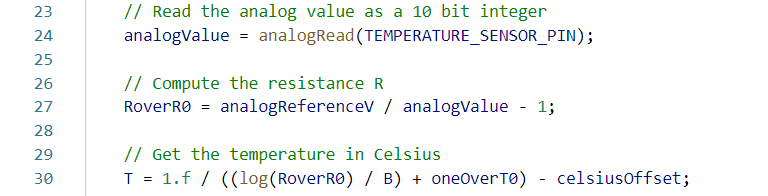
\includegraphics[width=0.9\textwidth]{temperature_compute.png}
    \caption*{\texttt{HW/part1/es05/temperature\_sensor.ino}: Intero codice per il calcolo della tem\-pe\-ra\-tu\-ra dalla lettura del sensore.}
    \label{fig:temp_compute}
\end{figure}

Infine, l'ultimo esercizio vede l'esordio del display 16x2. L'unità, pilotata tramite protocollo I\textsuperscript{2}C, è stata collegata ai pin corrispondenti sulla Arduino (SDA e SCL per i segnali di dato e clock, rispettivamente), mentre per quanto riguarda il software, ci siamo affidati alla libreria open source \textit{LiquidCrystal\_PCF8574}. Questa si è rivelata del tutto compatibile con il display in nostra dotazione, sebbene il comando \verb|LiquidCrystal_PCF8574::setBacklight(int brightness)| non è in grado di modificare l'effettiva luminosità dello schermo (come invece sembrerebbe dalla \textit{signature} del metodo), bensì ne può solamente determinare l'accensione dell'illuminazione o meno (questa sembrerebbe tuttavia essere una limitazione del particolare modello di display fornitoci, piuttosto che un difetto della libreria considerata).

\section{Seconda Parte}

\subsection{Configurazione Hardware}

Dopo aver letto i requisiti per il progetto dello \textit{smart home controller} (in versione locale), era chiaro che, rispetto alla parte precedente, bisognava apportare delle modifiche ai collegamenti:
\begin{enumerate}
    \item Il primo (e più ovvio) cambiamento, è stato sicuramente quello di dover utilizzare per la prima volta il sensore di rumore:
    dopo un veloce test del suo funzionamento, si è notato che tale sensore, anche se sottoposto ad un rumore apparentemente uniforme (in tono ed intensità), produce rapide oscillazioni sul suo output digitale.
    
    Per questo motivo, è impensabile utilizzare una strategia di \textit{polling} per la lettura di eventi di rumore, in quanto il sensore non fornisce un output stabile e deterministico per ogni rilevazione.
    
    Al contrario, il sensore di movimento è configurabile per tenere l'output alto (attivo) per un tempo variabile da 5 secondi a 5 minuti.
    
    Queste considerazioni, accoppiate al fatto che sulla Yùn il numero di pin di GPIO in grado di supportare interrupt esterni senza sacrificare altre funzionalità (o che non siano condivisi), è di fatto 1 (il pin numero 7), ci ha portato a scegliere di dedicare il privilegio di poter generare interrupt al sensore di rumore, mentre ci siamo accontentati del polling per il sensore PIR.
    
    Questo, in pratica, si è tradotto nel collegamento del sensore di rumore al pin di GPIO 7, mentre il sensore PIR è stato relegato al pin 13.
    
    La sensibilità del sensore di rumore, inoltre, è stata impostata in modo che non fosse attivato, per quanto possibile, dal rumore ambientale, pur mantenendo un buon compromesso rispetto al rilevamento della voce umana a qualche decina di centimetri di distanza.
    \item In secondo luogo, è stato necessario spostare il led rosso dal pin 12 utilizzato in precedenza per la prima parte del laboratorio, ad un pin che supportasse l'output PWM; nel nostro caso è stato scelto il pin 6.
\end{enumerate}
\noindent
Nella configurazione finale, ogni sensore ed attuatore fornitoci è stato usato, così come ogni cavetto \textit{jumper} ed entrambe le coppie di resistenze e led.

\subsection{Software}

Lo sviluppo dello sketch ha seguito la suddivisione in esercizi delineata nella traccia del laboratorio. La soluzione è organizzata su quattro file scritti dal gruppo: uno in formato \textit{.ino}, contenente i metodi \verb|setup()| e \verb|loop()| dello sketch, e tre librerie di supporto, che verranno descritte in seguito.
\\ \\
Il codice fa massiccio uso di variabili globali, che possono quindi essere condivise tra i vari metodi in modo diretto; inoltre, la maggior parte delle costanti sono dichiarate sotto forma di \verb|#define|, per ottimizzare l'utilizzo di memoria in runtime (molte sarebbero comunque state tradotte in costanti \textit{compile time} dal compilatore in ogni caso, probabilmente).
\\ \\
\verb|setup()| si occupa dell'inizializzazione delle risorse che verranno utilizzate dalla Yùn, come l'interfaccia seriale e il display I\textsuperscript{2}C, così come l'impostare i \textit{pin mode} per ogni periferica connessa alla stessa. Ogni variabile viene inizializzata in concomitanza con la sua dichiarazione, in ambito globale, perciò non è necessario farlo qui.
Infine, come anticipato nella sezione precedente, l'interrupt esterno collegato al sensore di rumore viene inizializzato in modalità \verb|FALLING|: il motivo di questa scelta deriva dal fatto che tale sensore è attivo basso, quindi al rilevamento di un segnale di rumore, il suo output si abbassa (si noti comunque che, per via della natura prettamente \textit{instabile} della linea in uscita da tale sensore osservata sperimentalmente, con ogni probabilità non si avrebbe ottenuto pressochè alcuna differenza pratica nel funzionamento dell'Arduino anche impostando l'interrupt in \verb|RISE|).
\\ \\
Il metodo \verb|loop()| è il cuore della logica dello sketch. Per permettere più subroutine indipendenti con periodi di esecuzione differenti, come quelle per la gestione di nuovi eventi di rumore, oppure la lettura di valori aggiornati dai sensori di temperatura e di movimento, così come l'effettuare lo \textit{switch} tra le due modalità di visualizzazione dello schermo, è stato adottato un meccanismo del tutto generale ed estensibile.

In principio venne valutata la possibilità di adoperare uno dei timer a bordo della Yùn stessa per generare interrupt con una certa temporizzazione (attraverso, per esempio, la libreria \textit{TimerOne}, già utilizzata durante la prima parte del laboratorio), ma ben presto gli svantaggi di tale approccio si fecero evidenti: una simile soluzione, infatti, è molto difficilmente scalabile a più un evento contemporaneo (nel senso di ottenere due o più serie di interrupt con periodi diversi), in quanto ciò richiederebbe l'implementazione di una logica non banale per la riprogrammazione del timer all'interno della ISR.

Piuttosto, la nostra soluzione esegue ogni subroutine in modo sincrono all'interno del ciclo \verb|loop()| stesso: per ogni procedura da eseguire nel ciclo, viene dichiarata una variabile globale \verb|unsigned long|, dedicata a contenere l'istante di tempo in millisecondi in cui l'ultima esecuzione del metodo corrispondente si è verificata (come \verb|timeOfLastLoopSensor| o \verb|timeOfLastLcdSwitch|). Ad ogni iterazione del \verb|loop()|, nella variabile locale \verb|unsigned long now| viene caricato l'istante attuale in millisecondi (funzione \verb|millis()|); successivamente, tale variabile viene confrontata con ognuna delle sue controparti globali descritte poco fa incrementate del rispettivo periodo, in modo da determinare se è necessario eseguire tale subroutine oppure no.
\begin{figure}[h]
    \centering
    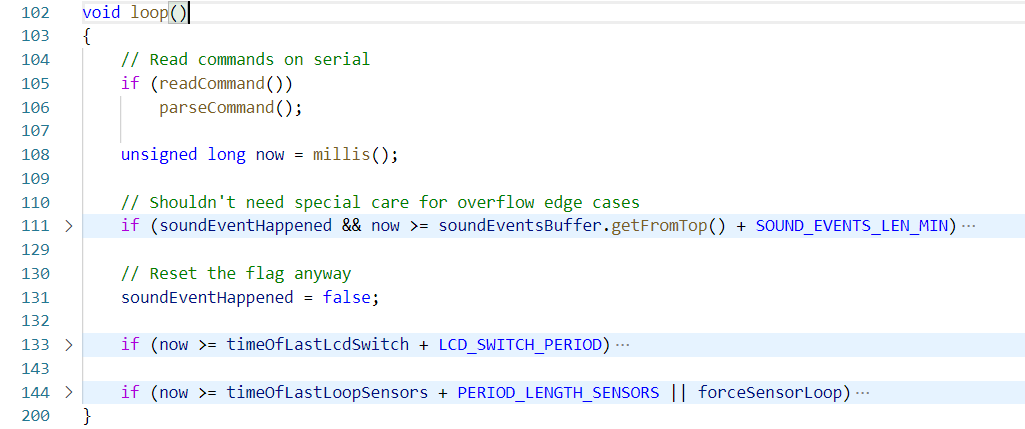
\includegraphics[width=0.9\textwidth]{loop_func.png}
    \caption*{\texttt{HW/part2/es2.8/es2.8.ino}: Funzione \texttt{loop()}.}
    \label{fig:loop_func}
\end{figure}
\subsubsection{Gestione degli eventi di rumore}

\textit{Le ISR devono essere il più corte e semplici possibili}. Questo è un principio fondamentale nel mondo embedded, ed in particolare in quello Arduino. La pagina ufficiale della documentazione riferita al metodo \verb|attachInterrupt(...)| (\url{https://www.arduino.cc/reference/en/language/functions/external-interrupts/attachinterrupt/}) così recita: \textit{Generally, an ISR should be as short and fast as possible.}
\\ \\
Le motivazioni di una tale filosofia sono molteplici; tanto per cominciare, di default il microcontrollore a bordo delle schede Arduino non supporta interrupt annidati (all'interno di una ISR è possibile abilitarli manualmente, ma sembra essere una pratica sconsigliata), il che impone che, durante l'esecuzione di una \textit{Interrupt Service Routine}, nient'altro può avvenire. Per esempio, il contatore che si occupa di incrementare l'output di \verb|millis()| si affida ad un interrupt interno.
\\ \\
Proprio in funzione di questo \textit{design language} si è deciso, per questa applicazione, di trasferire ogni computazione dalla ISR al loop principale, che viene comunque eseguito di continuo senza delay intermedi grazie all'approccio sopra descritto.

Di fatto, il metodo \verb|noiseSensorISR()| setta un flag globale e \verb|volatile|, il quale viene continuamente campionato in \verb|loop()|, proprio come ogni altra subroutine.

Non ogni invocazione di \verb|noiseSensorISR()|, infatti, deve corrispondere ad un \textit{evento di rumore} nel senso dell'esercizio: il sensore produce, per ogni suono di intensità sufficiente, moltissimi eventi distinti in rapidissima successione, che non rappresentano, singolarmente, una distinta unità di rumore secondo la logica del programma. Per questo, un semplice check scarta tutti gli eventi generati dal sensore che distano meno di una certa soglia dall'evento precedente (durante i nostri test, settare \verb|SOUND_EVENTS_LEN_MIN| a \SI{500}{\milli\second} si è rivelato sufficientemente efficacie).
\\ \\
Per implementare la finestra progressiva di accumulazione dei sample, è stata implementata una semplice \textit{deque} ad array circolare (file \textit{HW/part2/utils/IntegerArrayDeque.hpp}). Tale struttura è essenzialmente una coda \textit{LIFO} accessibile da entrambi i lati, ed inizializzata con una dimensione pari a \verb|SOUND_EVENTS_MIN|. In questo modo, ad ogni nuovo evento di rumore, il suo timestamp viene inserito in testa al buffer, mentre un ciclo \verb|while| scorre la coda dal fondo, eliminando ogni elemento avvenuto almeno \verb|soundInterval| millisecondi fa.

Se, al termine di tale procedura, la struttura è piena, il flag booleano \verb|personSound| viene settato a true.
\begin{figure}[htbp]
    \centering
    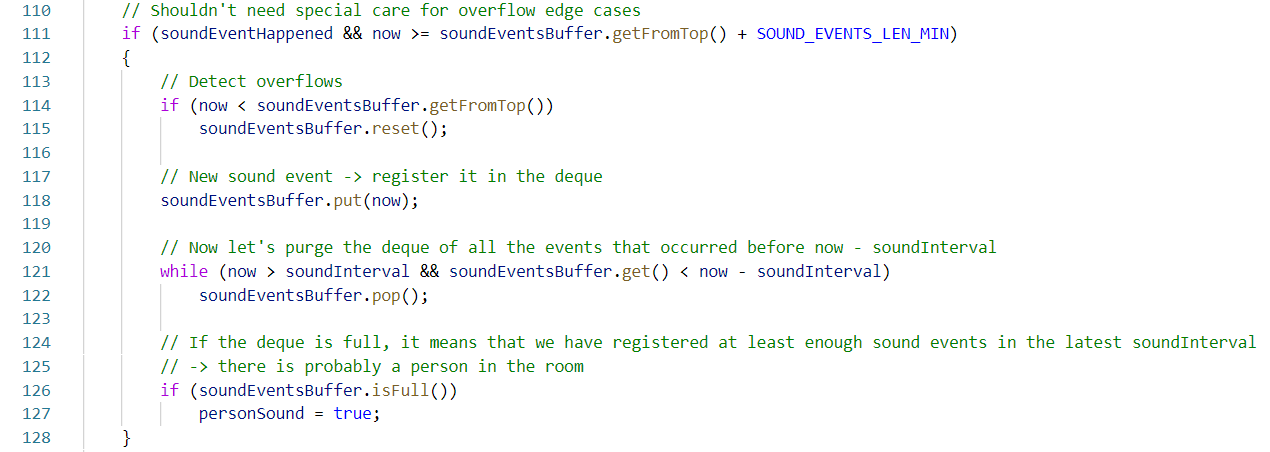
\includegraphics[width=0.9\textwidth]{sound.png}
    \caption*{\texttt{HW/part2/es2.8/es2.8.ino}: Gestione degli eventi di rumore.}
    \label{fig:sound}
\end{figure}

\subsubsection{Rilevamento di persone}

Ogni \verb|PERIOD_LENGTH_SENSORS| millisecondi (due secondi e mezzo nei nostri test) viene eseguito il campionamento dei sensori di temperatura e movimento. Se quest'ultimo rileva una presenza, la corrispettiva \verb|personPir| viene settata; se al contrario l'ultimo trigger del sensore è avvenuto prima di \verb|timeoutPir| millisecondi fa, il flag viene impostato a zero. La stessa logica è implementata per il sensore di rumore.
%TODO: Inserire codice

A questo punto, i contributi dei due sensori sono semplicemente uniti in \verb|OR| logico ad ottenere la globale \verb|person|, indicatrice di presenza, o meno, di una persona nella stanza.

\subsubsection{Temperatura, riscaldamento e condizionamento}

\begin{figure}[h]
    \centering
    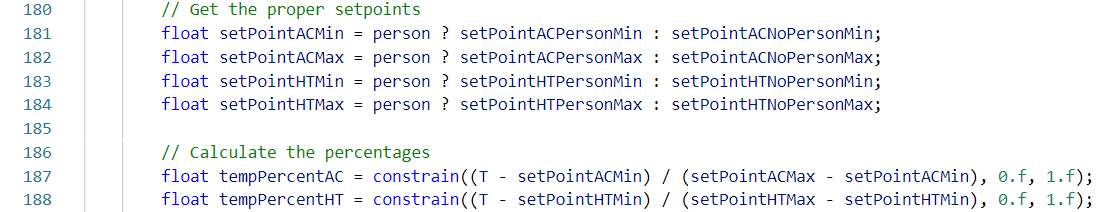
\includegraphics[width=0.9\textwidth]{set_points.png}
    \caption*{\texttt{HW/part2/es2.8/es2.8.ino}: Calcolo delle percentuali di attuazione relative ai \textit{set point}.}
    \label{fig:set_points}
\end{figure}

Il programma mantiene due coppie di range di temperatura, per l'attivazione delle unità di riscaldamento (il led rosso), e di condizionamento (la ventola), nelle varianti con o senza rilevamento di una persona.
\\ \\
immediatamente dopo aver aggiornato il valore di \verb|person|, l'Arduino sceglie la giusta coppia di \textit{set point}, dopodiché calcola le percentuali rappresentate dalla temperatura corrente rispetto ai range di temperature \verb|setPointAC[Min/Max]| e \verb|setPointHT[Min/Max]| tramite la seguente formula:
$$percent = \frac{T-rangeLow}{rangeHigh-rangeLow}$$
\\ \\
I valori così ottenuti, poi ristretti tra 0 e 1 e riscalati su $[0,255]$, vengono passati alle rispettive \verb|analogWrite(...)| per imporre il corretto duty cycle ad entrambe le uscite PWM.

\subsubsection{Output sul display \texorpdfstring{I\textsuperscript{2}C}{i2c}}

La gestione dello schermo sfrutta le funzioni definite nel file \textit{HW/part2/utils/Display\-Utils.hpp}. I suddetti metodi sono stati spostati in un file separato puramente per ragioni di ordine del codice, ma le funzioni stesse si appoggiano su variabili globali, quindi l'inclusione di questa \textit{``libreria''} (il termine qui è usato in modo improprio), così come per \textit{CommandParserUtils.hpp}, avviene successivamente alla dichiarazione di tali variabili.
\\ \\
Il display presenta due possibili modalità di visualizzazione che si scambiano ogni \verb|LCD_SWITCH_PERIOD| millisecondi.

Il contenuto visualizzato sullo schermo, in ogni momento, può essere suddiviso in due sottogruppi:
\begin{itemize}
    \item \textbf{contenuto statico}: comprende caratteri e parole che rimangono invariati durante l'intero periodo per cui rimane a schermo. In particolare, questo significa punteggiatura ed etichette.
    \item \textbf{contenuto dinamico}: tutta la parte di dati, come la temperatura attuale, set point impostati correntemente, e la percentuale di operatività dei moduli di riscaldamento e condizionamento.
\end{itemize}

La distinzione si è resa utile per ottimizzare l'invio di dati tramite il bus I\textsuperscript{2}C, un'operazione particolarmente costosa.
In pratica, ad ogni switch della modalità di visualizzazione, viene aggiornato il contenuto statico (funzione \verb|printStaticContentLCD()|, che si riferisce alla variabile booleana globale \verb|lcdStatus|), mentre il contenuto dinamico è aggiornato, in funzione della modalità attuale dello schermo, dopo ogni lettura di valori dei sensori e conseguente aggiornamento dei parametri del programma (funzione \verb|updateDynamicContentLCD(...)|).

Si può comprendere quindi l'utilità di \verb|forceSensorLoop|, che è usata per \textit{forzare} l'esecuzione della subroutine di lettura dei sensori (e quindi aggiornamento dei contenuti dinamici del display) il più presto possibile, in modo da popolare immediatamente lo schermo dopo l'accensione dell'Arduino.

\subsubsection{Gestione dell'interfaccia seriale}

Poiché i comandi per l'aggiornamento dei range di temperatura devono essere più lunghi di un singolo carattere, è stato adottato un approccio differente rispetto a quello implementato nella prima parte del laboratorio.
\\ \\
Il formato scelto per permettere l'impostazione dei set point è così strutturato
\begin{center}
    \verb|usp <set-point to update> <min> <max>|
\end{center}
Dove \verb|usp| sta per \verb|Update Set Point|, mentre i possibili set point da aggiornare sono identificabili da
\begin{itemize}
    \item \verb|ac| o \verb|acp|: i set point relativi al controllo del condizionamento, rispettivamente senza oppure con la rilevazione di una persona;
    \item \verb|ht| o \verb|htp|: analogo al caso precedente per il riscaldamento.
\end{itemize}
Infine, \verb|<min>| e \verb|<max>| devono essere numeri in virgola mobile rappresentanti gli estremi dell'intervallo di temperatura. Tra una parola e l'altra è possibile inserire un numero arbitrario di spazi.
\\ \\
La funzionalità si basa sul buffer globale \verb|cmd|; ad ogni iterazione del loop principale, la funzione \verb|readCommand()| legge tutti i byte dall'interfaccia seriale finchè viene trovato il carattere \verb|'\n'|, e li carica su \verb|cmd|. Se il \textit{newline} non è presente, i byte messi in \verb|cmd| vengono considerati parte di un comando incompleto, e non verranno sovrascritti alla successiva chiamata di \verb|readCommand()|. Al termine della lettura, se il buffer risulta pieno, il suo intero contenuto viene scartato, in quanto il comando sarebbe probabilmente errato. Letto \verb|'\n'|, invece, gli si sostituisce immediatamente il terminatore di stringa \verb|'\0'|, e viene chiamata la \verb|parseCommand()|.
\\ \\
Tramite l'uso di un paio di funzioni di supporto per gestire gli eventuali spazi all'interno della stringa, quest'ultima usa il metodo \verb|strncmp(...)| per confrontare le sottostringhe del comando con le sequenze di caratteri attese.

Infine, i valori in virgola mobile rappresentanti i nuovi set point sono letti tramite la \verb|atof(...)|, e un messaggio di aggiornamento avvenuto con successo è stampato.

\subsection{Bonus}

Grazie alla struttura adottata per interpretare gli eventi di rumore per le richieste precedenti, gran parte della soluzione dell'esercizio bonus era, di fatto, già implementata.
\\ \\
Infatti, l'idea che sta dietro al funzionamento di un \textit{identificatore di battiti consecutivi} tramite un così semplice sensore di rumore, si fonda sul rilevare due segnali con una temporizzazione compatibile con due battiti di mani: è necessario, cioè, definire un intervallo di tempo - per ogni segnale rilevato - entro il quale, in caso di ulteriore evento di rumore, deve essere acceso il led.

In pratica, due eventi troppo vicini tra loro devono essere scartati, e allo stesso modo due segnali eccessivamente distanti nel tempo non costituiscono un doppio battito. Durante le nostre prove, abbiamo individuato l'intervallo di tempo $[150, 500]$ \si{\milli\second} essere particolarmente efficacie (costanti \verb|SOUND_EVENTS_LEN_MIN| e \verb|SOUND_EVENTS_LEN_MAX|).
\\ \\
Alcune considerazioni: questo metodo, seppur decisamente grezzo, funziona in modo sorprendentemente convincente per quanto riguarda la rilevazione della sequenza desiderata; il suo più grande problema, a nostro parere, è quello dei falsi positivi che, troppo facilmente, riescono ad ingannare il sistema: è sufficiente soffiare sul sensore per far lampeggiare il led, ed in generale qualsiasi rumore di durata sufficiente e che sia abbastanza intenso, verrà scambiato per due battiti di mani consecutivi.

\section{Terza Parte}

Gli ultimi esercizi dei laboratori dedicati all'hardware si concentrano sugli aspetti legati all'Internet della piattaforma Arduino di cui siamo dotati. Questo comprende, quindi, rispondere a richieste HTTP, eseguirle, oppure scambiare messaggi tramite il protocollo MQTT.

\subsection{3.1 - Yùn come server HTTP}

L'Arduino Yun contiene due processori: il primo - più semplice - dedicato all'esecuzione di codice Arduino, che ha accesso alle interfacce di I/O, più un secondo processore che, tra le altre cose, si occupa di gestire la connessione ad Internet.
\\ \\
La comunicazione tra questi due chip avviene tramite un componente chiamato \textit{Bridge}, ovvero un'interfaccia seriale dedicata.
L'ambiente di sviluppo Arduino mette perciò a disposizione una API che permette di inizializzare tale interfaccia, nonché utilizzarla per svolgere funzioni di alto livello.
\\ \\
In particolare, questo primo esercizio si basa sulle classi \verb|BridgeServer| e \verb|BridgeClient|:
nella funzione \verb|setup()| viene inizializzato il server attraverso un oggetto di tipo \verb|BridgeServer|; dopodichè, in \verb|loop()|, viene eseguito il polling periodico di tale oggetto per processare ogni connessione in ingresso.

\noindent Quest'ultimo punto, in particolare, viene svolto dalla funzione \verb|processConnection(...)|, che accetta un argomento di tipo \verb|BridgeClient|.
\\ \\
Così come per gli esercizi successivi, per la (de)codifica dei documenti in formato JSON, ci si è affidati alla libreria open-source \textit{ArduinoJson} che, a costo di una maggiore dimensione del codice compilato, permette una notevole astrazione, nonché semplificazione, della gestione di tale tipologia di documenti.

\subsection{3.2 - Yùn come client HTTP}

In modo molto simile all'esercizio precedente, per eseguire richieste HTTP da codice Arduino, ci si avvale del bridge della Yùn per poter sfruttare le funzionalità del processore Linux a bordo della scheda.
\\ \\
Questa volta, però, viene usata la classe \verb|Process|, che ha scopo molto più ampio e generale di ciò per cui viene usata qui, infatti permette di eseguire comandi generici del sistema Linux in esecuzione sul coprocessore della Yùn, e riceverne il risultato. In questo caso, lanciamo il comando \verb|curl|, un programma molto potente in ambiente Linux, al quale passiamo i parametri adeguati per eseguire richieste \verb|POST| presso un server nella rete locale.

\begin{figure}[h]
    \centering
    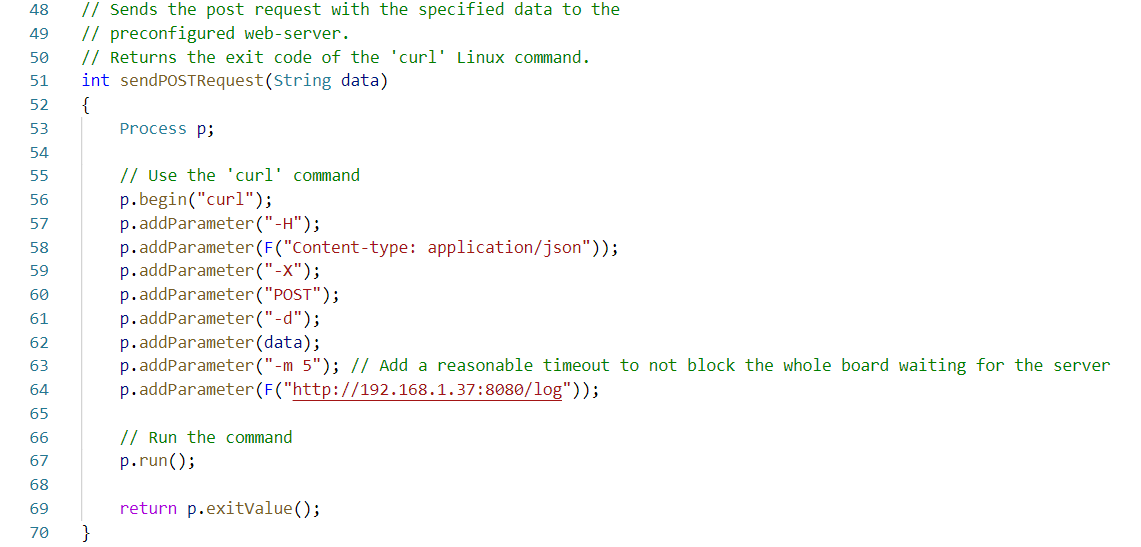
\includegraphics[width=0.9\textwidth]{post.png}
    \caption*{\texttt{HW/part3/es3.2/es3.2.ino}: Esecuzione del comando \texttt{post} sul coprocessore Linux tramite \texttt{Process}.}
    \label{fig:post}
\end{figure}

Anche questa volta, il loop principale è molto semplice, e si limita a eseguire la lettura del valore analogico riportato dal sensore di temperatura, convertire tale lettura in una temperatura, nonché utilizzarla per creare un documento JSON tramite \textit{ArduinoJson}, per infine inviare tale documento al server in ascolto. (Per quanto riguarda il server, si rimanda alla descrizione degli esercizi 1-2 del primo laboratorio software)

\subsection{3.3 - Yùn come client MQTT}

Infine, l'ultimo esercizio prevede di utilizzare la Yùn per scambiare messaggi in MQTT. Per fare ciò, abbiamo seguito il consiglio del professor Pagliari impiegando la libreria \textit{MQTTclient.h}, che permette di includere comunicazioni MQTT con pochissime righe di codice astraendo allo sviluppatore gli aspetti di più basso livello riguardanti \verb|Process|.

Al contrario di quanto era stato detto a lezione, tuttavia, si è rivelato necessario installare la suite \verb|mosquitto| sul processore Linux della board, in quanto non risultava preinstallata \textit{out-of-the-box}.
\\ \\
In ogni caso, il codice è anche questa volta piuttosto eloquente, tuttavia questo esercizio si è rivelato, in fase di sviluppo, la prima istanza in cui si sono presentati problemi riconducibili alla scarsa quantità di memoria installata a bordo della Yùn.
Per questo motivo, è possibile notare piccole differenze rispetto agli esercizi precedenti, volti proprio a cercare di diminuire l'uso di memoria dinamica necessaria; un esempio di ciò a cui mi sto riferendo può essere il limite più stretto scelto per la dimensione degli oggetti \verb|DynamicJsonDocument|, oppure il tentativo di ridurre al minimo l'uso di \verb|String|, sostituito, nella funzione \verb|encodeSenML(...)|, da un buffer allocato dinamicamente.
\\ \\
I problemi a cui ci si riferisce sono, per esempio, l'invio di messaggi MQTT vuoti, oppure la scorretta deserializzazione di documenti JSON, eccetera...

Alla fine, comunque, si è scoperto che l'uso esagerato di memoria da parte di uno sketch apparentemente molto semplice era da imputarsi ad uno scorretto uso della libreria \verb|MQTTclient.h|: sbadatamente, nelle prime implementazioni dell'esercizio, veniva infatti creata una nuova istanza della classe \verb|MQTTclient|, ignorando l'esistenza dell'istanza default nella variabile \verb|mqtt|; la risoluzione di questo errore ha portato alla liberazione di una significativa porzione di memoria del codice, nonché, finalmente, al corretto funzionamento dello sketch.
\\ \\
Ad ogni modo, comunque, simili problemi si ripresenteranno in seguito negli esercizi facenti parte dei laboratori software, in cui la soluzione non sarà, ahimè, così banale. Piuttosto, si è dovuto impiegare pratiche quali l'affidamento della pubblicazione del JSON di sottoscrizione al device catalog ad uno script sh nella memoria del processore Linux, il quale veniva semplicemente richiamato tramite la libreria \verb|Process| dallo sketch.
\end{document}
